\documentclass[sigconf,nonacm]{acmart}

\settopmatter{printacmref=false}
\renewcommand\footnotetextcopyrightpermission[1]{}

\usepackage{booktabs}
\usepackage{array}
\usepackage{tabularx}
\usepackage{dblfloatfix}
\usepackage{float}
\usepackage{tikz}
\usepackage{xspace}
\usetikzlibrary{arrows.meta,positioning,fit,shapes.geometric}

\newcolumntype{L}[1]{>{\raggedright\arraybackslash}p{#1}}
\newcolumntype{Y}{>{\raggedright\arraybackslash}X}

\newcommand{\briskstate}{BriskState\xspace}

\title{Demonstrating \briskstate: A Cache-Aware State Backend for Apache Flink}

\author{Anonymous Authors}
\affiliation{%
  \institution{Anonymous Submission}%
  \city{Anonymous}%
  \country{Anonymous}%
}

\begin{document}

\begin{abstract}
State-intensive stream processing often becomes memory-bound before it becomes compute-bound. Frequent state lookups, window maintenance, and timer firing amplify cache misses, long object-indirection chains, and heap-management overhead, making state-backend efficiency a first-order performance concern. We present \briskstate, an Apache Flink state backend that combines a thin Java control layer, a JNI bridge, and a native execution engine to reorganize keyed state around compact, locality-aware structures. This demo shows how these design choices improve over heap-based state backends on the official Flink state-backend JMH suite and on a seven-workload benchmark set. The demo supports side-by-side execution and compact runtime summaries so that throughput, tail latency, and state-access differences can be tied back to backend organization under identical workloads.
\end{abstract}

\keywords{stream processing, Apache Flink, keyed state, in-memory state backend, memory locality}

\maketitle

\section{Introduction}
State-intensive stream-processing pipelines rely on the state backend on nearly every record. In Apache Flink, this path is exercised by point updates, window aggregation, joins, and timer callbacks, so backend behavior can dominate end-to-end performance even when user logic is lightweight \cite{carbone2015flink}. In practice, the bottleneck is frequently the memory hierarchy rather than arithmetic throughput: state accesses trigger pointer chasing, touch multiple cache lines, and create runtime jitter through heap-management activity. This is directly relevant to parallel processing because modern streaming jobs scale out compute across many task slots while repeatedly converging on shared bottlenecks in the memory hierarchy. When each parallel task repeatedly exercises stateful operators, poor locality amplifies cache and TLB pressure, introduces tail-latency spikes, and makes additional cores less effective than their nominal count suggests. A backend that preserves locality on the state path therefore improves not just raw throughput, but also how well a multicore deployment sustains parallel speedups under skewed and state-heavy workloads.

We present \briskstate, a cache-aware Flink state backend designed to improve state-access locality in state-intensive workloads. \briskstate keeps Flink integration in a thin Java control layer and moves keyed-state lookup, routing, and storage into a native engine reached through JNI. The demo compares BriskState against heap-based backends on identical workloads and highlights how compact state layout and locality-aware access paths affect throughput, tail latency, and state-access behavior. Rather than presenting only final summary numbers, we relate those measurements to the backend's main design ideas: a lightweight native implementation, namespace grouping, and cache-friendly indexing aimed at reducing cache misses on the critical state path.

\briskstate is positioned against three nearby lines of work. Stateful dataflow systems such as MillWheel, Flink, Naiad, Structured Streaming, and the Dataflow model define high-level execution semantics, but the physical organization of state remains largely hidden behind operator APIs and runtime services \cite{akidau2013millwheel,carbone2015flink,murray2013naiad,armbrust2018structured,akidau2015dataflow}. In Flink deployments, backend choices usually reduce to in-memory heap structures or embedded persistent stores such as RocksDB, while work on consistent state management and migration, including Flink state management and Megaphone, emphasizes correctness and continuity rather than layout-aware backend optimization \cite{carbone2015flink,rocksdb,carbone2017statemanagement,hoffman2019megaphone}. High-performance key-value engines and compact hash-table designs, including FASTER and Swiss-table-style indexing, show that memory layout and probing discipline materially change access cost, while application mixes such as the seven topologies revisited by Zhang et al. expose how operator structure interacts with modern multicore hardware \cite{chandramouli2018faster,abseil2018swisstable,zhang2017revisiting}. \briskstate targets this gap by implementing a Flink-compatible state backend whose layout-driven optimizations deliver measurable gains over heap-based alternatives on both microbenchmark and application workloads.

This paper makes three contributions:
\begin{itemize}
  \item It presents \briskstate as a Flink-compatible cache-aware state backend built from a Java control layer, a JNI bridge, and a native execution engine.
  \item It demonstrates, using the official Flink state-backend microbenchmark and a seven-workload benchmark set, that \briskstate improves throughput and tail latency over standard heap-based baselines.
  \item It provides a compact demonstration methodology that links observed gains to key-group routing, namespace partitioning, and compact native storage.
\end{itemize}

\section{\briskstate}
\subsection{Overview}
Figure~\ref{fig:architecture} summarizes the implemented \briskstate architecture together with the companion demo UI used in the demonstration. The left side shows the execution stack from Flink runtime to the state engine; the right side shows the demo interface used for benchmark submission, cluster configuration, and runtime throughput and latency display.

The figure distinguishes the execution stack from the presentation layer. Flink integration and serializer analysis stay in Java, while keyed-state storage, namespace partitioning, and snapshot consistency move into the state engine. The demo UI is shown separately because it is used to configure the cluster, submit benchmark runs, and display runtime throughput and latency during the demonstration. The underlying storage path follows compact, cache-conscious hash-table ideas inspired by modern Swiss-table designs \cite{abseil2018swisstable}, and those choices are precisely what drive BriskState's gains over heap-based baselines.

\begin{figure}[H]
  \centering
  
\includegraphics[width=\columnwidth]{../fig1.png}
  \caption{BriskState architecture and the companion demo UI. The left side shows the execution path from Flink runtime through the Java control layer and JNI bridge into the native state engine, where key-group routing, namespace partitioning, compact storage, and snapshot/restore are implemented. The right side shows the control surface used in the demonstration to submit workloads, compare backends, and inspect runtime throughput and latency under the same deployment.}
  \Description{A layered architecture image showing Flink runtime, Java control layer, JNI bridge, and state engine on the left, with a companion Demo UI panel on the right for benchmark submission, cluster configuration, throughput, and latency display.}
  \label{fig:architecture}
\end{figure}

That systems view maps cleanly to the implemented storage hierarchy. At the backend level, state is partitioned first by key-group and then by namespace before it reaches a compact sub-table. When the namespace is the common void namespace used by many keyed operators, the extra namespace map can be skipped and the backend addresses one table per key-group directly; otherwise each key-group owns a namespace-to-table map, and empty namespaces are removed eagerly after clears. This design reduces routing overhead on the hot path while keeping state isolation explicit enough to visualize per-namespace skew during the demonstration.

BriskState is evaluated with two workload families. The first is the official Flink \texttt{flink-state-benchmark} JMH suite for state backends, which isolates per-operation ValueState, ListState, and MapState costs under controlled loops. The second is our seven-workload benchmark set, adapted from the task mix in Zhang et al. \cite{zhang2017revisiting}, that combines fan-out, fan-in, and branch-merge topologies to stress state routing under more application-like pipelines. Together, they show where BriskState's backend design pays off, from isolated state operations to end-to-end streaming jobs.

\subsection{Evaluation Setup}
\briskstate is evaluated with Flink-compatible state management, the official Flink state-backend JMH suite, and the seven-workload benchmark set used for end-to-end comparison. The evaluation therefore builds on real workloads and measured results rather than on a synthetic front end alone. Table~\ref{tab:setup} summarizes the experimental platform used for both the microbenchmark and the end-to-end Flink runs.

\begin{table*}[t]
  \caption{Experimental setup.}
  \label{tab:setup}
  \centering
  \footnotesize
  \begin{tabularx}{\textwidth}{L{0.2\textwidth}Y}
    \toprule
    Item & Configuration \\
    \midrule
    Hardware platform & Intel Xeon Platinum 8368Q x86\_64 server, 38 physical cores / 76 hardware threads, 251~GiB memory \\
    Software stack & Linux, Apache Flink, and the implemented \briskstate backend \\
    Flink deployment & One JobManager and two TaskManagers for controlled side-by-side backend comparison \\
    TaskManager config & Four slots per TaskManager with 16~GiB process memory per TaskManager \\
    Default parallelism & 8 \\
    \bottomrule
  \end{tabularx}
\end{table*}

\briskstate also remains faster at the operator level. Across the 13 retained \texttt{flink-state-benchmark} operations, the largest gains appear on list iteration (+132\%), map insertion (+110\%), map lookup (+91\%), value insertion (+87\%), and map removal (+74\%). These measurements come from the official Flink state-backend JMH benchmark rather than a separate operator-level application benchmark, so they isolate the state-access path directly. The pattern is consistent with the backend design: operations that repeatedly traverse lists, probe maps, or update compact keyed entries benefit most when pointer chasing and boxing overhead are reduced. Within the demonstration, these results therefore serve not only as a stable microbenchmark reference before the evaluation moves to larger job graphs, but also as evidence that the backend's locality-oriented layout materially changes the cost of common keyed-state operations.

The demo is organized in four stages:
\begin{enumerate}
  \item select a workload and switch between heap-based and cache-aware backends;
  \item compare time-series changes in throughput, tail latency, and backend-specific counters;
  \item examine which key-groups and namespaces receive the most accesses and how occupancy evolves;
  \item compare metrics and state summaries across repeated runs.
\end{enumerate}

This evaluation framing keeps the emphasis on how BriskState's layout decisions translate into visible gains over heap-based backends, from isolated state operations to full application pipelines. Our seven-workload benchmark set covers Stateful Word Count (WC), Fraud Detection (FD), Spike Detection (SD), Traffic Monitoring (TM), Log Processing (LG), Spam Detection in VoIP (VS), and Linear Road (LR). Adapted from the topology mix in Zhang et al. \cite{zhang2017revisiting}, it exercises \briskstate under the same Flink deployment. Figure~\ref{fig:benchset} shows 1.11$\times$--1.50$\times$ higher throughput per core on six workloads, with parity on VS. This spread is plausible given the topology mix: workloads with frequent keyed updates and repeated state probes leave more room for layout-driven savings, whereas pipelines whose cost is dominated by other operator work expose less headroom for the backend alone to improve overall throughput. The important point for the demo is therefore not that every workload improves by the same margin, but that the direction of the gain remains stable across several different branch and merge structures.

\begin{figure*}[t]
  \centering
  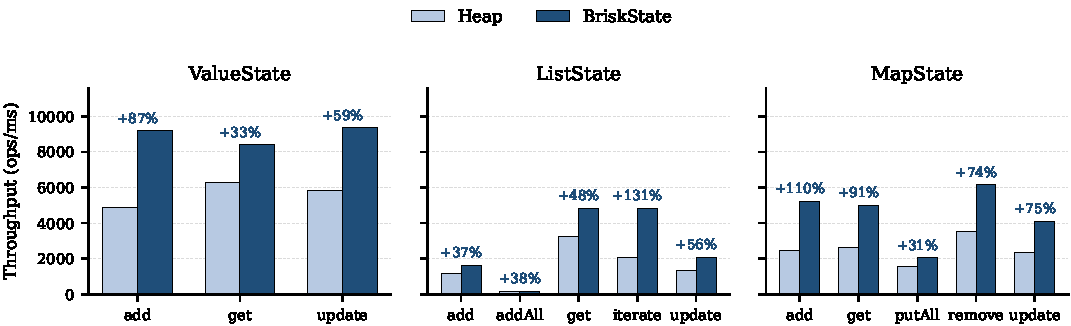
\includegraphics[width=0.9\textwidth]{flink_state_benchmark_intel.pdf}
  \caption{Results from the official Flink \texttt{flink-state-benchmark} JMH suite on our local experiment setup. \briskstate outperforms the heap backend across retained ValueState, ListState, and MapState operations.}
  \Description{A three-panel grouped bar chart showing local-host microbenchmark throughput for ValueState, ListState, and MapState operations, with \briskstate above the heap baseline and speedup labels for each operation.}
  \label{fig:microbench}
\end{figure*}

\begin{figure}[t]
  \centering
  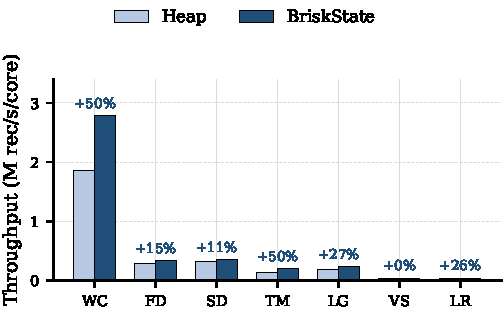
\includegraphics[width=\columnwidth]{benchset_throughput_paper.pdf}
  \caption{Throughput per core on our seven-workload benchmark set. \briskstate improves six of the seven application pipelines and matches the heap baseline on the VoIP spam-detection workload.}
  \Description{A compact grouped bar chart comparing HashMapStateBackend and BriskState throughput per core for the seven benchmark-set workloads WC, FD, SD, TM, LG, VS, and LR.}
  \label{fig:benchset}
\end{figure}

\subsection{Runtime Support}
The runtime support is intentionally simple. The UI lets the operator configure the cluster, submit benchmark runs, choose the state backend, and view throughput and latency in real time. These functions keep the interaction focused on backend comparison rather than on auxiliary tooling. The demonstration therefore uses the interface as a thin control and reporting surface: it launches the same workloads under different backends and presents the resulting measurements in a consistent format across repeated runs.

\begin{figure*}[t]
  \centering
  \resizebox{0.97\textwidth}{!}{%
  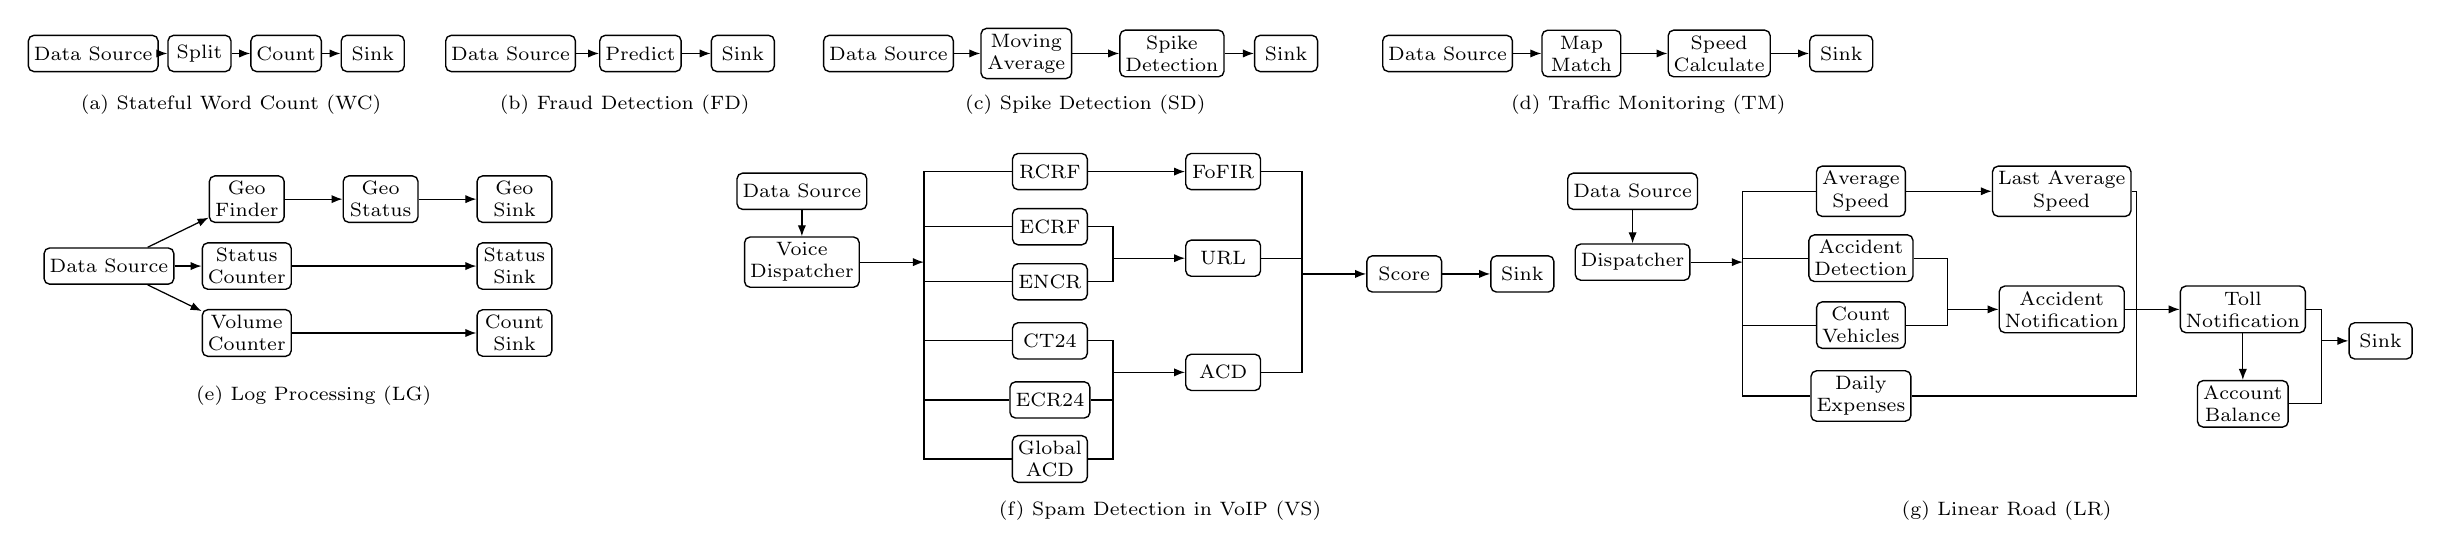
\begin{tikzpicture}[
      font=\scriptsize,
      topo/.style={draw, rounded corners=2pt, line width=0.5pt, fill=white, align=center, minimum height=0.46cm, inner sep=2pt},
      flow/.style={-{Latex[length=1.4mm]}, line width=0.45pt},
      collect/.style={line width=0.45pt},
      label/.style={font=\scriptsize},
      title/.style={font=\scriptsize\bfseries},
      chip/.style={draw, rounded corners=1.5pt, line width=0.4pt, fill=white, inner sep=2pt}
    ]
    \node[topo, minimum width=1.2cm] (wcsrc) at (0.8,4.8) {Data Source};
    \node[topo, minimum width=0.8cm] (wcsplit) at (2.15,4.8) {Split};
    \node[topo, minimum width=0.8cm] (wccount) at (3.25,4.8) {Count};
    \node[topo, minimum width=0.8cm] (wcsink) at (4.35,4.8) {Sink};
    \draw[flow] (wcsrc) -- (wcsplit);
    \draw[flow] (wcsplit) -- (wccount);
    \draw[flow] (wccount) -- (wcsink);
    \node[label] at (2.55,4.15) {(a) Stateful Word Count (WC)};

    \node[topo, minimum width=1.2cm] (fdsrc) at (6.1,4.8) {Data Source};
    \node[topo, minimum width=0.95cm] (fdpred) at (7.75,4.8) {Predict};
    \node[topo, minimum width=0.8cm] (fdsink) at (9.05,4.8) {Sink};
    \draw[flow] (fdsrc) -- (fdpred);
    \draw[flow] (fdpred) -- (fdsink);
    \node[label] at (7.55,4.15) {(b) Fraud Detection (FD)};

    \node[topo, minimum width=1.2cm] (sdsrc) at (10.9,4.8) {Data Source};
    \node[topo, minimum width=1.15cm] (sdma) at (12.65,4.8) {Moving\\Average};
    \node[topo, minimum width=1.1cm] (sdspike) at (14.5,4.8) {Spike\\Detection};
    \node[topo, minimum width=0.8cm] (sdsink) at (15.95,4.8) {Sink};
    \draw[flow] (sdsrc) -- (sdma);
    \draw[flow] (sdma) -- (sdspike);
    \draw[flow] (sdspike) -- (sdsink);
    \node[label] at (13.4,4.15) {(c) Spike Detection (SD)};

    \node[topo, minimum width=1.2cm] (tmsrc) at (18.0,4.8) {Data Source};
    \node[topo, minimum width=1.0cm] (tmmap) at (19.7,4.8) {Map\\Match};
    \node[topo, minimum width=1.0cm] (tmspeed) at (21.45,4.8) {Speed\\Calculate};
    \node[topo, minimum width=0.8cm] (tmsink) at (23.0,4.8) {Sink};
    \draw[flow] (tmsrc) -- (tmmap);
    \draw[flow] (tmmap) -- (tmspeed);
    \draw[flow] (tmspeed) -- (tmsink);
    \node[label] at (20.55,4.15) {(d) Traffic Monitoring (TM)};

    \node[topo, minimum width=1.2cm] (lgsrc) at (1.0,2.1) {Data Source};
    \node[topo, minimum width=0.95cm] (lggeo) at (2.75,2.95) {Geo\\Finder};
    \node[topo, minimum width=0.95cm] (lgstatus) at (2.75,2.1) {Status\\Counter};
    \node[topo, minimum width=0.95cm] (lgvolume) at (2.75,1.25) {Volume\\Counter};
    \node[topo, minimum width=0.95cm] (lggeost) at (4.45,2.95) {Geo\\Status};
    \node[topo, minimum width=0.95cm] (lgsinka) at (6.15,2.95) {Geo\\Sink};
    \node[topo, minimum width=0.95cm] (lgsinkb) at (6.15,2.1) {Status\\Sink};
    \node[topo, minimum width=0.95cm] (lgsinkc) at (6.15,1.25) {Count\\Sink};
    \draw[flow] (lgsrc) -- (lggeo);
    \draw[flow] (lgsrc) -- (lgstatus);
    \draw[flow] (lgsrc) -- (lgvolume);
    \draw[flow] (lggeo) -- (lggeost);
    \draw[flow] (lggeost) -- (lgsinka);
    \draw[flow] (lgstatus) -- (lgsinkb);
    \draw[flow] (lgvolume) -- (lgsinkc);
    \node[label] at (3.6,0.45) {(e) Log Processing (LG)};

    \node[topo, minimum width=1.2cm] (vssrc) at (9.8,3.05) {Data Source};
    \node[topo, minimum width=1.2cm] (vsdisp) at (9.8,2.15) {Voice\\Dispatcher};
    \node[topo, minimum width=0.95cm] (vsrcrf) at (12.95,3.3) {RCRF};
    \node[topo, minimum width=0.95cm] (vsecrf) at (12.95,2.6) {ECRF};
    \node[topo, minimum width=0.95cm] (vsencr) at (12.95,1.9) {ENCR};
    \node[topo, minimum width=0.95cm] (vsct24) at (12.95,1.15) {CT24};
    \node[topo, minimum width=0.95cm] (vsecr24) at (12.95,0.4) {ECR24};
    \node[topo, minimum width=0.95cm] (vsgacd) at (12.95,-0.35) {Global\\ACD};
    \node[topo, minimum width=0.95cm] (vsfofir) at (15.15,3.3) {FoFIR};
    \node[topo, minimum width=0.95cm] (vsurl) at (15.15,2.2) {URL};
    \node[topo, minimum width=0.95cm] (vsacd) at (15.15,0.75) {ACD};
    \node[topo, minimum width=0.95cm] (vsscore) at (17.45,2.0) {Score};
    \node[topo, minimum width=0.8cm] (vssink) at (18.95,2.0) {Sink};
    \draw[flow] (vssrc) -- (vsdisp);
    \coordinate (vsbus) at (11.35,2.15);
    \draw[flow] (vsdisp.east) -- (vsbus);
    \foreach \target in {vsrcrf,vsecrf,vsencr,vsct24,vsecr24,vsgacd} {\draw[collect] (vsbus) |- (\target.west);}
    \draw[flow] (vsrcrf) -- (vsfofir);
    \coordinate (vsurlmerge) at (14.2,2.2);
    \draw[collect] (vsecrf.east) -- (13.75,2.6) |- (vsurlmerge);
    \draw[collect] (vsencr.east) -- (13.75,1.9) |- (vsurlmerge);
    \draw[flow] (vsurlmerge) -- (vsurl.west);
    \coordinate (vsacdmerge) at (14.2,0.75);
    \draw[collect] (vsct24.east) -- (13.75,1.15) |- (vsacdmerge);
    \draw[collect] (vsecr24.east) -- (13.75,0.4) |- (vsacdmerge);
    \draw[collect] (vsgacd.east) -- (13.75,-0.35) |- (vsacdmerge);
    \draw[flow] (vsacdmerge) -- (vsacd.west);
    \coordinate (vsscoremerge) at (16.65,2.0);
    \draw[collect] (vsfofir.east) -- (16.15,3.3) |- (vsscoremerge);
    \draw[collect] (vsurl.east) -- (16.15,2.2) |- (vsscoremerge);
    \draw[collect] (vsacd.east) -- (16.15,0.75) |- (vsscoremerge);
    \draw[flow] (vsscoremerge) -- (vsscore.west);
    \draw[flow] (vsscore) -- (vssink);
    \node[label] at (14.35,-1.0) {(f) Spam Detection in VoIP (VS)};

    \node[topo, minimum width=1.2cm] (lrsrc) at (20.35,3.05) {Data Source};
    \node[topo, minimum width=1.0cm] (lrdisp) at (20.35,2.15) {Dispatcher};
    \node[topo, minimum width=1.0cm] (lravg) at (23.25,3.05) {Average\\Speed};
    \node[topo, minimum width=1.0cm] (lrlast) at (25.8,3.05) {Last Average\\Speed};
    \node[topo, minimum width=1.0cm] (lracc) at (23.25,2.2) {Accident\\Detection};
    \node[topo, minimum width=1.0cm] (lrcount) at (23.25,1.35) {Count\\Vehicles};
    \node[topo, minimum width=1.0cm] (lrdaily) at (23.25,0.45) {Daily\\Expenses};
    \node[topo, minimum width=1.05cm] (lrnotify) at (25.8,1.55) {Accident\\Notification};
    \node[topo, minimum width=1.0cm] (lrtoll) at (28.1,1.55) {Toll\\Notification};
    \node[topo, minimum width=1.0cm] (lracct) at (28.1,0.35) {Account\\Balance};
    \node[topo, minimum width=0.8cm] (lrsink) at (29.85,1.15) {Sink};
    \draw[flow] (lrsrc) -- (lrdisp);
    \coordinate (lrbus) at (21.75,2.15);
    \draw[flow] (lrdisp.east) -- (lrbus);
    \foreach \target in {lravg,lracc,lrcount,lrdaily} {\draw[collect] (lrbus) |- (\target.west);}
    \draw[flow] (lravg) -- (lrlast);
    \coordinate (lrnotifymerge) at (24.95,1.55);
    \draw[collect] (lracc.east) -- (24.35,2.2) |- (lrnotifymerge);
    \draw[collect] (lrcount.east) -- (24.35,1.35) |- (lrnotifymerge);
    \draw[flow] (lrnotifymerge) -- (lrnotify.west);
    \coordinate (lrtollmerge) at (27.2,1.55);
    \draw[collect] (lrlast.east) -- (26.75,3.05) |- (lrtollmerge);
    \draw[collect] (lrnotify.east) -- (lrtollmerge);
    \draw[collect] (lrdaily.east) -- (26.75,0.45) |- (lrtollmerge);
    \draw[flow] (lrtollmerge) -- (lrtoll.west);
    \draw[flow] (lrtoll) -- (lracct);
    \coordinate (lrsinkmerge) at (29.1,1.15);
    \draw[collect] (lrtoll.east) -- (29.1,1.55) |- (lrsinkmerge);
    \draw[collect] (lracct.east) -- (29.1,0.35) |- (lrsinkmerge);
    \draw[flow] (lrsinkmerge) -- (lrsink.west);
    \node[label] at (25.1,-1.0) {(g) Linear Road (LR)};
  \end{tikzpicture}%
  }
  \caption{Topologies in the seven-workload benchmark set, adapted from Zhang et al. \cite{zhang2017revisiting}. The set spans seven stateful pipelines with different branch, merge, and routing structure.}
  \Description{Seven compact pipeline diagrams showing the benchmark-set workloads: Stateful Word Count, Fraud Detection, Spike Detection, Traffic Monitoring, Log Processing, Spam Detection in VoIP, and Linear Road.}
  \label{fig:benchset-topology}
\end{figure*}

\section{Demonstration Scenario}
The demonstration begins with a side-by-side comparison mode. One workload is executed with two different backends, and the synchronized dashboard reports throughput, latency percentiles, and backend-specific counters. This mode establishes that BriskState improves not only final job time but also runtime stability and responsiveness. It provides a direct view of how backend choice alone alters the steady-state execution profile under the same workload.

The second stage connects the optimization back to state layout directly. The interface renders a hierarchical view from operator to key-group to namespace, then overlays heat and occupancy information to show where accesses concentrate. This view shows how a smaller and more stable working set appears when namespaces are separated into compact sub-tables, and how that change corresponds to the throughput and latency gains seen in comparison runs. At this point, the operator can switch workloads or inspect a specific high-activity key-group, allowing the demo to move from aggregate metrics to a structural explanation of where the saved work comes from.

The demonstration steps through two workload families under the same dashboard: the official Flink state-backend benchmark suite for per-operation state costs, and the seven-workload benchmark set for application pipelines with richer branching and merging structure. This sequence answers two increasingly demanding questions: whether the gain persists on isolated Flink state operations, and whether the same trend survives in multi-operator pipelines with branch and merge structure.

Figure~\ref{fig:benchset-topology} explains why the benchmark set is more informative than a single monolithic query: some pipelines are short and update-dense, some branch into multiple keyed paths, and others merge several stateful summaries before the sink.

Using the same dashboard across these workload families also keeps the comparison disciplined. The operator does not switch between unrelated measurement tools when moving from operator-level microbenchmarks to end-to-end streaming jobs; instead, the same reporting surface is reused so that changes in throughput, latency, and state summaries can be interpreted as backend effects rather than as artifacts of a different measurement path.

The demonstration workflow is intentionally lightweight but concrete. The operator can choose the next workload family, rerun the same job under the heap baseline, and compare throughput and latency summaries against the previous run. Because the same scripts and deployment layout are reused throughout the session, the workflow remains focused on backend behavior rather than on one-off tuning. The demo therefore communicates not only that BriskState is faster on these Intel experiments, but also why the improvement is reproducible across both operator and application views.

\section{Discussion and Conclusion}
State backends are central to modern stream processing, but their key properties are physical rather than logical. \briskstate turns those physical choices into measurable gains through compact native storage, locality-aware access paths, and a Flink-compatible integration layer. The resulting demonstration connects backend design directly to throughput gains and lower latency over heap-based backends. By combining the native state backend, the evaluation workloads, workload control, and synchronized metrics, the demo compares \briskstate directly against heap-based baselines under the same workloads and shows that state layout materially affects performance and stability.

The gains instead come from three coordinated design ideas. First, \briskstate adopts a lightweight native state-backend implementation so that the hot state path is not dominated by Java-object indirection and heap-management overhead. Second, it groups state by namespace, which makes routing and access more regular under repeated keyed operations. Third, it uses a cache-friendly indexing structure so that lookups and updates touch a smaller and more stable working set. These choices serve the same objective: reducing cache misses on the critical state-access path. That is why the improvements are most visible on update-heavy and lookup-heavy operations, yet still remain observable across richer end-to-end pipeline topologies.

The contribution of the paper is therefore not only to present a working Flink-compatible backend, but also to show how these implementation choices can be inspected under a common evaluation path spanning both operator-level and application-level workloads. The demonstration supports that goal by keeping workload control, backend selection, and metric reporting in one workflow, so that performance differences can be related back to concrete structural choices in the backend rather than treated as isolated benchmark outcomes.

\balance
\bibliographystyle{ACM-Reference-Format}
\bibliography{briskstate-demo}

\end{document}